\chapter{Visitor}

E' un pattern \underline{comportamentale}, descrive come classi e oggetti interagiscono e si distribuiscono le responsabilità. 
\smallskip

Consente di definire una nuova operazione senza modificare le classi degli oggetti su cui opera ed è utile quando si ha una gerarchia di classi e si desidera eseguire 
diverse operazioni su di esse senza dover aggiungere nuovi metodi a ciascuna classe (le operazioni variano a seconda del tipo di classe concreta).

\section{Funzionamento}

Avremo un'interfaccia comune, AbstractVisitor, che definisce metodi del tipo visitXXX per ogni tipo \underline{concreto} della struttura e le sottoclassi concrete che 
estendono AbstractVisitor.

Nella classe base/interfaccia della gerarchia aggiungiamo il metodo accept(...) che prende in input un AbstractVisitor e le classi concrete della gerarchia 
implementeranno tale metodo chiamando il corrispettivo metodo visitXXX passando se stesso come input.
\medskip

\textbf{N.B.} Questo pattern sopperisce alla mancanza del \underline{double dispatch}  (overloading dinamico).
\medskip

Supponiamo di prendere in considerazione l'esempio dell'esercitazione Expression.

Quindi avremo la nostra interfaccia ExpressionVisitor con due metodi, visitConstant e visitSum che prendono in input, rispettivamente, un Constant ed un Sum e una sua 
implementazione concreta, ParenthesisRepresentationVisitor. 

Nell'interfaccia Expression avremo il metodo accept(...) che prende in input ExpressionVisitor ed infine avremo le classi Constant e Sum che implementeranno accept(...) 
chiamando rispettivamente visitConstant e visitSum.

\section{Double dispatch}

Supponiamo di avere il seguente test

\begin{lstlisting}
@Test
public void testReprImproved() {
    ExpressionVisitor r = new ParenthesisRepresentationVisitor();
    Expression exp = new Sum(
                        new Constant(10),
                        new Constant(5)
                        );
    assertEquals("(10 + 5)", exp.accept(r));
}
\end{lstlisting}

Quando chiamiamo exp.accept(r), exp, staticamente, è di tipo Expression ma a runtime è di tipo Sum e quindi, per il binding dinamico, viene chiamato visitSum.

VisitSum, staticamente, prende in input un oggetto di tipo ExpressionVisitor che, a runtime, è di tipo ParenthesisRepresentationVisitor, quindi per il binding dinamico, 
viene chiamato ParenthesisRepVisitor.visitSum.

Ecco perchè double dispatch, ovvero abbiamo usato due volte il meccanismo del binding dinamico.

\section{Perchè si arriva al Visitor}

\subsection{Overloading statico}
Prendiamo sempre come esempio expression e definiamo la classe ParenthesisRepresentation che implementa il metodo repr in overloading, uno accetta Sum e l'altro 
Constant che ritorna un stringa.
\begin{lstlisting}
public class ParenthesisRepresentation {
  
  public String repr(Constant c) {
    return "Constant";
  }
  
  public String repr(Sum s) {
    return "Sum";
  }
}   
\end{lstlisting}

Supponiamo ora che vogliamo migliorare i metodi, il primo ritorna il valore della constante in stringa, mentre il secondo deve rappresentare l'operazione di 
somma di due valori.
\begin{lstlisting}
public class ParenthesisRepresentation {
  public String repr(Constant c) {
    return "" + c.getValue();
  }

  public String repr(Sum s) {
    return "(" +
            repr(s.getLeft()) +
            " + " +
            repr(s.getRight()) +
            ")";
  }
}
\end{lstlisting}

Il compilatore ci segnalerà due warning in repr(Sum s) perchè i metodi getLeft() e getRight() ritornano un Expression e noi non abbiamo un metodo repr che 
accetta un expression.

Quindi aggiungiamo il terzo metodo repr che lancia un eccezione perchè noi pensiamo che non venga mai chiamata
\begin{lstlisting}
public String repr(Expression expr) {
  throw new UnsupportedOperationException("Caso non contemplato");
}   
\end{lstlisting}

ed invece verrà chiamata perchè i i metodi getLeft() e getRight() ritornano un Expression e, siccome l'overloading è statico, viene chiamato repr(Expression expr).

\subsection{Simulare l’overloading dinamico con un dispatch manuale}

Prendiamo il metodo repr(Expression expr) e usiamo instanceof e cast
\begin{lstlisting}
public class ParenthesisRepresentation {
  public String repr(Expression expr) {
    if (expr instanceof Constant) {
      return repr((Constant) expr);
    } else if (expr instanceof Sum) {
      return repr((Sum) expr);
    }
    throw new UnsupportedOperationException("Caso non contemplato");
  }
  
  public String repr(Constant c) {...}
  public String repr(Sum s) {...}
}
\end{lstlisting}

tutto ok ma il tutto è macchinoso e poco leggibile, usiamo instanceof e cast (che è “error prone”), è inefficiente e c'è lo spauracchio dell'eccezione dietro l'angolo.

Infatti se passiamo Multipliction, avremo eccezione.

\subsection{dispatch map}

Quindi usiamo una Map per selezionare il metodo in base al tipo effettivo dell’oggetto dove Key: Class, Value: lambda che chiama il metodo
\begin{lstlisting}
public class ParenthesisRepresentation {
  private Map<Class<? extends Expression>,Function<Expression, String>> dispatchMap = new HashMap<>();

  public ParenthesisRepresentation() {
    dispatchMap.put(Constant.class, e -> repr((Constant) e));
    dispatchMap.put(Sum.class, e -> repr((Sum) e));
  }

  public String repr(Expression expr) {
    Function<Expression, String> method = dispatchMap.get(expr.getClass());
    if (method == null)
      throw new UnsupportedOperationException("Caso non contemplato");
    return method.apply(expr);
  }
  public String repr(Constant c) {...}
  public String repr(Sum s) {...}
}
\end{lstlisting}

Molto difficile da implementare e mantenere, ci sono sempre i downcast che sono error-pronee c’è sempre la possibilità dell’UOException, e più facile compiere 
imprecisazioni o sviste di codice però è più efficiente del dispatch manuale.

\section{Collaborazioni}

\begin{figure}[H]
  \centering
  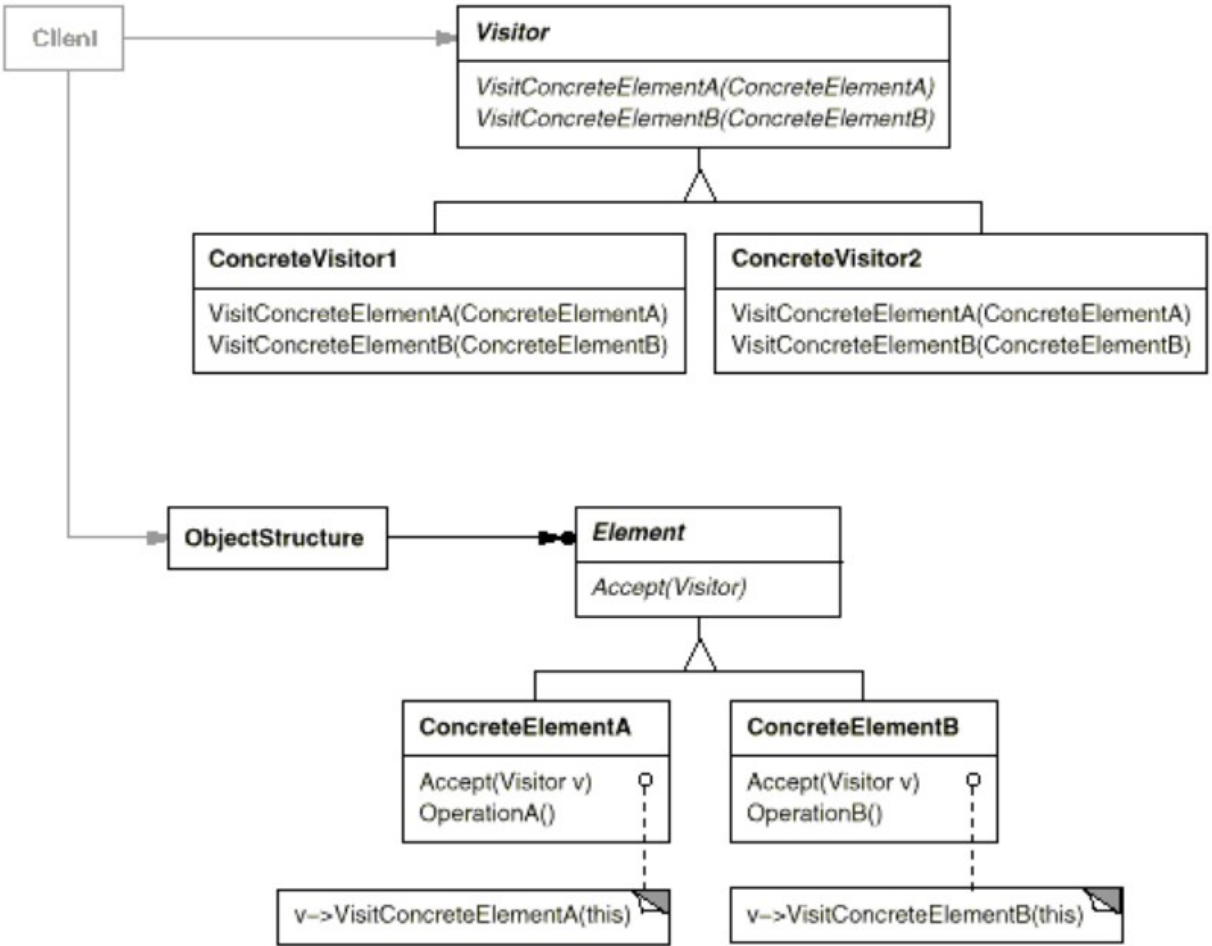
\includegraphics[width=8cm]{../../immagini/visitor/struttura_visitor}
\end{figure}

Un client crea un ConcreteVisitor e visita la struttura a oggetti.

Quando un elemento viene visitato chiama il metodo del visitor che corrisponde alla sua classe, passando se stesso come argomento, in questo modo il visitor può 
accedere allo stato dell’oggetto, se necessario.
\smallskip

Aggiungere una nuova classe alla gerarchia, come Multipliction, comporterà aggiungere un nuovo metodo visitXXX, in ExpressionVisitor, che prenderà in input 
Multipliction ed implentare accept(...) in Multipliction e l'aggiunta di questo metodo comporterà errori di compilazione nei visitor concreti, quindi occorrerà 
implementarlo.

\section{Varianti Visitor}

Supponiamo di voler rimuovere il metodo eval() da Expression e di implementare la valutazione di un espressione tramite il EvalVisitor, tale che 
EvalVisitor$<:$ExpressionVisitor.

\subsection{Visitor generico}

Dall'esempio precendete, noi sappiamo che in ExpressionVisitor i metodi visitXXX ritornano una stringa, ma a noi servirebbe che i metodi visitXXX di EvalVisitor 
ritornino un integer, quindi rendiamo ExpressionVisitor generico e, a sua volta, i metodi visitXXX e accept diventeranno generici.

Andremo a specificare l'argomento di tipo solamente quando andremo ad implementare Expression, con ParenthesisRepresentationVisitor o EvalVisitor, e nei test, in quanto
non possiamo instanziare in tipo generico, instanziamo direttamente il visitor concreto.

\subsection{Visitor void}

I metodi visitXXX e accept sono void e per questo motivo ogni visitor concreto si deve mantere uno stato, che viene usato per accumulare i risultati durante la visita, 
ed infine fornire un metodo per ottenere il risultato finale di tutta la vista.

\section{Coseguenze}

Affinchè i visitor possano agire sugli elementi, l'interfaccia degli elementi deve fornire operazioni pubbliche di accesso e questo compromette l'incapsulamento.

E' facile aggiungere nuove operazioni, basta aggiungere un visitor concreto.

E' difficile aggiungere un nuovo elemento da visitare, bisogna definire un nuovo metodo in visitor che poi dovrà essere implementato dalle classi concrete e il nuovo 
elemento da visitare deve implementare accept.

Per questo motivo, il visitor andrebbe usato quando la gerarchia degli oggetti è \underline{stabile}.

Una soluzione a questo, potrebbe essere quella di fornire un'implementazione dei metodi visitXXX in una classe astratta che implementa Visitor, cosicchè i client che 
implementeranno Visitor, estenderanno la classe astratta e ridefiniranno i metodi di loro interesse (questo però è un altro pattern).

Simulando il binding dinamico, facciamo a meno di instanceof e downcast.

Inoltre, se il linguaggio permettesse l'overloading dinamico, allora non ci sarebbe bisogno del metodo accept nelle classi da visitare ma comunque, quest'ultime, 
dovrebbero sempre fornire punti di accesso alla classe.